\documentclass[tikz,border=3pt]{standalone}
\usepackage{fontspec}
\usepackage{amsmath}
\usepackage{xcolor}
\usepackage{tikz}
\usepackage{pgfplots}
\pgfplotsset{compat=1.18}
\usetikzlibrary{arrows.meta,calc,fit,positioning,shapes.geometric,shapes.misc,patterns,plotmarks}
\IfFontExistsTF{Arial}{\setsansfont{Arial}}{\setsansfont{TeX Gyre Heros}}
\renewcommand{\familydefault}{\sfdefault}
\tikzset{
  >={Stealth[length=2.2mm,width=1.5mm]},
  exact title/.style={font=\bfseries\fontsize{10.5}{12}\selectfont,align=center},
  exact subtitle/.style={font=\fontsize{6.3}{7.2}\selectfont,align=center},
  exact label/.style={font=\fontsize{6.4}{7.5}\selectfont,align=center},
  exact tiny/.style={font=\fontsize{5.3}{6.3}\selectfont,align=center},
  panel/.style={draw=black!14,rounded corners=1.2mm,fill=white,line width=.45pt},
  neutral/.style={draw=black!30,fill=black!3,rounded corners=1mm,line width=.45pt},
  arrow/.style={-Stealth,line width=.7pt},
  softarrow/.style={-Stealth,line width=.55pt,draw=black!45},
  dashedarrow/.style={-Stealth,dashed,line width=.55pt,draw=black!55},
  metric/.style={font=\fontsize{5.3}{6.3}\selectfont,fill=white,inner sep=1pt},
}
\newcommand{\pill}[4]{\node[draw=#2!70,fill=#2!10,rounded corners=1.5mm,inner xsep=3pt,inner ysep=2pt,exact label,text=#2] (#1) at #3 {#4};}
\newcommand{\frameboxx}[4]{\draw[draw=#2!65,fill=#2!8,rounded corners=.6mm,line width=.5pt] (#1.south west) rectangle (#1.north east);\node[exact tiny,text=#2] at #3 {#4};}
\newcommand{\axislabel}[3]{\node[exact tiny,text=black!60] at (#1) {#2};\node[exact tiny,text=black!60,rotate=90] at (#3) {#2};}

\definecolor{oviolet}{HTML}{6D597A}\definecolor{oorange}{HTML}{F28F3B}\definecolor{oteal}{HTML}{2A9D8F}\definecolor{oblack}{HTML}{263238}\definecolor{ogrid}{HTML}{A7B0B7}
\begin{document}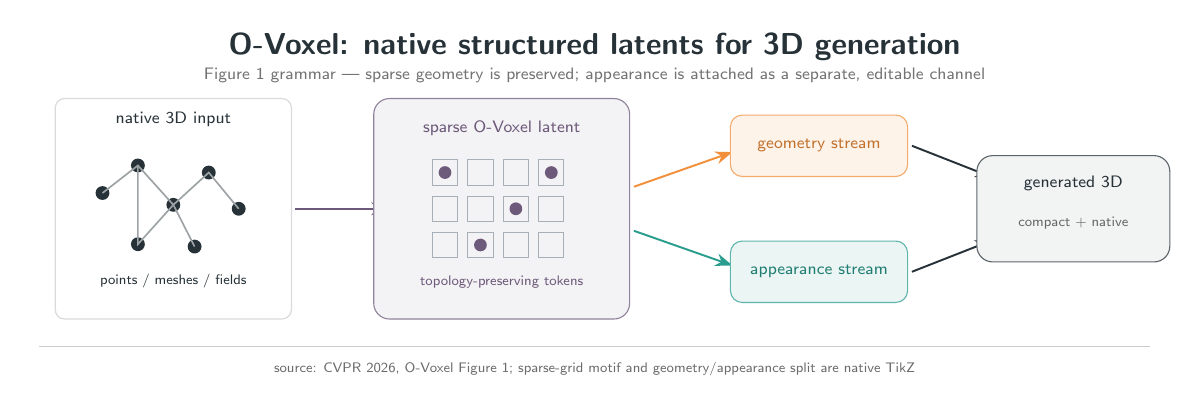
\begin{tikzpicture}[x=1cm,y=1cm]
\path[use as bounding box] (-.2,-2.3) rectangle (14.2,2.3);
\node[exact title,text=oblack] at (7,2.05) {O-Voxel: native structured latents for 3D generation};
\node[exact subtitle,text=black!55] at (7,1.7) {Figure 1 grammar — sparse geometry is preserved; appearance is attached as a separate, editable channel};
\node[panel,minimum width=3.0cm,minimum height=2.8cm] (input) at (1.65,0) {};
\node[exact label,text=oblack] at (1.65,1.14) {native 3D input};
\foreach \x/\y in {.75/.2,1.2/.55,1.65/.05,2.1/.46,2.48/.0,1.2/-.45,1.92/-.48}{\fill[oblack] (\x,\y) circle (2.5pt);}
\draw[oblack!45,line width=.6pt] (.75,.2)--(1.2,.55)--(1.65,.05)--(2.1,.46)--(2.48,0);\draw[oblack!45,line width=.6pt] (1.2,.55)--(1.2,-.45)--(1.65,.05)--(1.92,-.48);
\node[exact tiny,text=oblack] at (1.65,-.92) {points / meshes / fields};
\draw[arrow,draw=oviolet] (3.2,0) -- (4.38,0);
\node[draw=oviolet!75,fill=oviolet!8,rounded corners=2mm,minimum width=3.25cm,minimum height=2.8cm] (voxel) at (5.82,0) {};
\node[exact label,text=oviolet] at (5.82,1.02) {sparse O-Voxel latent};
\foreach \x/\y in {5.1/.46,5.55/.46,6/.46,6.45/.46,5.1/0,5.55/0,6/0,6.45/0,5.1/-.46,5.55/-.46,6/-.46,6.45/-.46}{\draw[ogrid,line width=.35pt] (\x-.16,\y-.16) rectangle (\x+.16,\y+.16);}
\foreach \x/\y in {5.1/.46,6/0,5.55/-.46,6.45/.46}{\fill[oviolet] (\x,\y) circle (2.3pt);}
\node[exact tiny,text=oviolet] at (5.82,-.93) {topology-preserving tokens};
\draw[arrow,draw=oorange] (7.5,.28) -- (8.75,.72);\draw[arrow,draw=oteal] (7.5,-.28) -- (8.75,-.72);
\node[draw=oorange!75,fill=oorange!11,rounded corners=1.5mm,minimum width=2.25cm,minimum height=.78cm,exact label,text=oorange!80!black] at (9.85,.8) {geometry stream};
\node[draw=oteal!75,fill=oteal!10,rounded corners=1.5mm,minimum width=2.25cm,minimum height=.78cm,exact label,text=oteal!80!black] at (9.85,-.8) {appearance stream};
\draw[arrow,draw=oblack] (11.03,.8) -- (12.05,.4);\draw[arrow,draw=oblack] (11.03,-.8) -- (12.05,-.4);
\node[draw=oblack!75,fill=oblack!6,rounded corners=2mm,minimum width=2.45cm,minimum height=1.35cm] (out) at (13.08,0) {};
\node[exact label,text=oblack] at (13.08,.32) {generated 3D};\node[exact tiny,text=black!60] at (13.08,-.18) {compact + native};
\draw[black!20,line width=.45pt] (-.05,-1.75) -- (14.05,-1.75);
\node[exact tiny,text=black!58] at (7,-2.03) {source: CVPR 2026, O-Voxel Figure 1; sparse-grid motif and geometry/appearance split are native TikZ};
\end{tikzpicture}\end{document}
